\documentclass[10pt,a4paper]{article}
\usepackage[utf8]{inputenc}
\usepackage{amsmath}
\usepackage{amsfonts}
\usepackage{amssymb}
\usepackage{listings}
\usepackage{graphicx}

\begin{document}
\title{Intelligent Systems Assignment 1}
\author{Wessel Becker (1982362) \& Sander ten Hoor (2318555)}
\maketitle
\section{MatLab code}
\subsection{Changes to tsp.m}
\subsection{plotmean.m}
\lstinputlisting[language=Matlab]{./Salesman/plotmean.m}

\section{Plots}
To show the impact of T, several T values have been used to run the tsp function. The tsp function returns the generated distance values. The last fifty of these values are used to plot the mean against the used T value.


These plots show the value of T on the x-axis against the mean on the y-axis. The standard deviation is displayed around the data points.


\makebox[\textwidth]{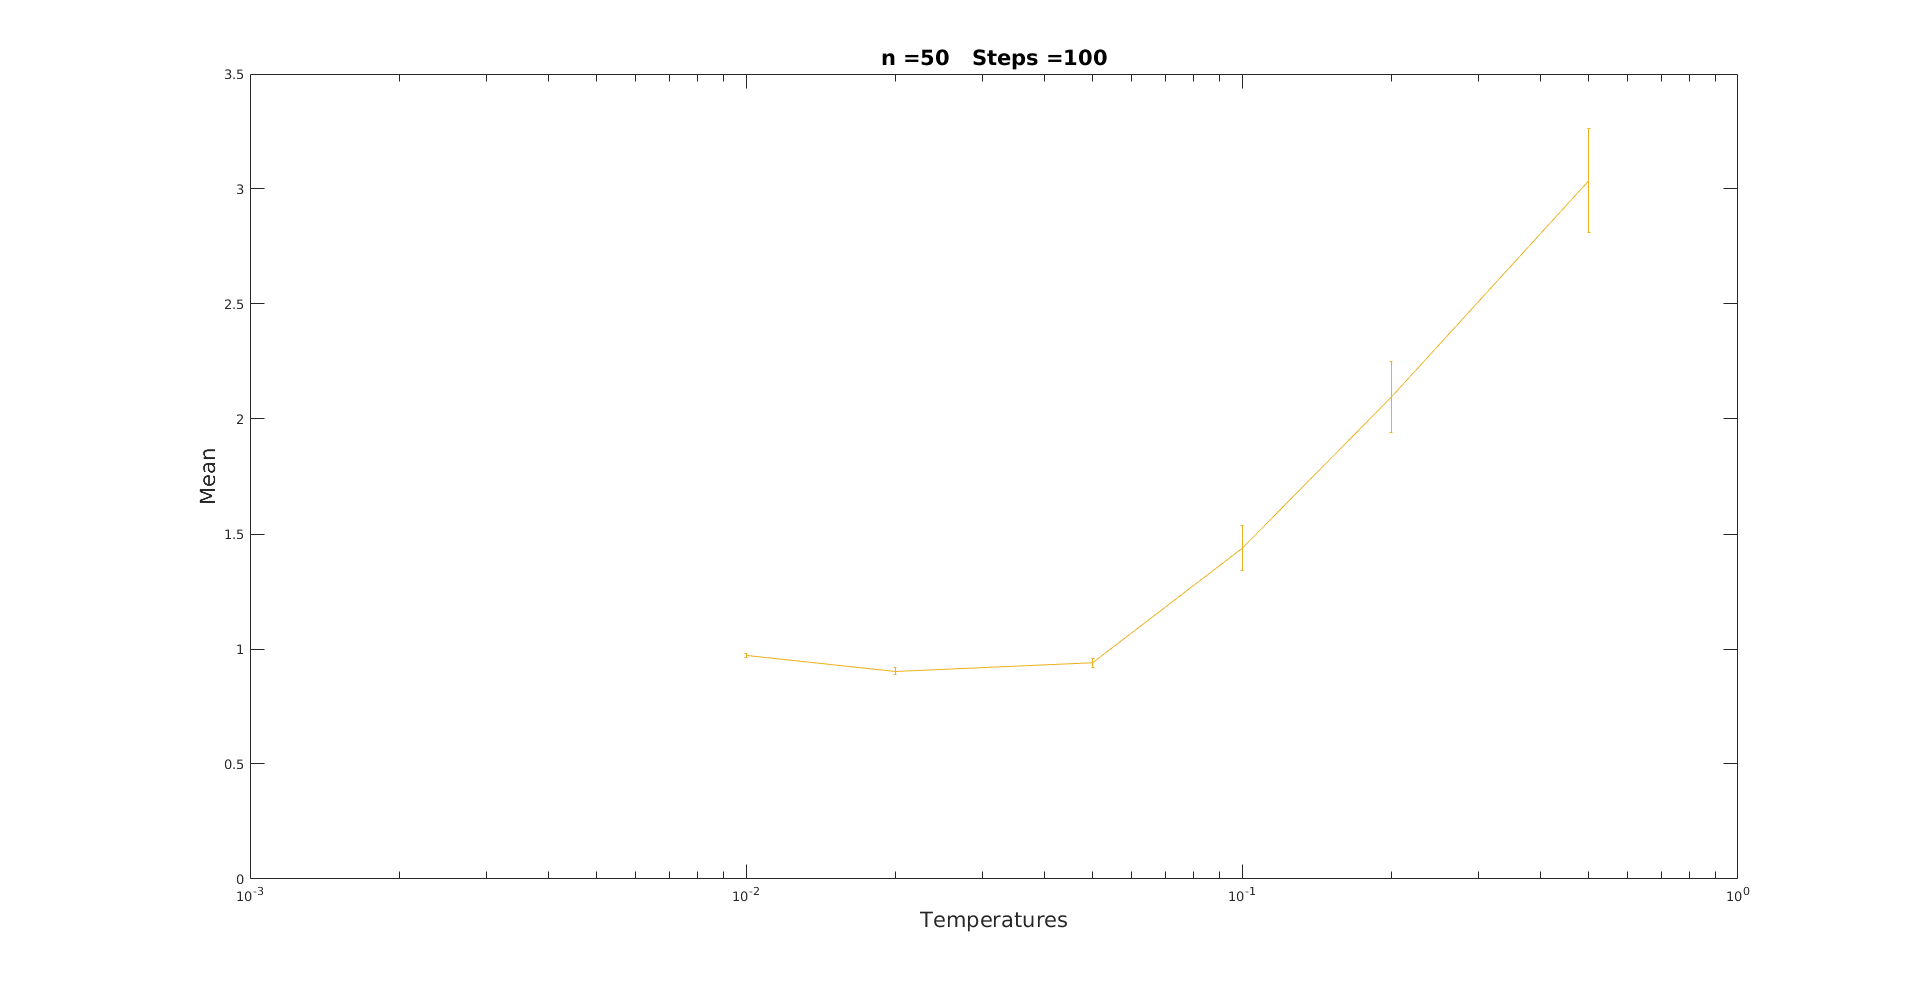
\includegraphics[width=\paperwidth]{./Salesman/n50steps100}}
\section{T-Dependance}
\section{Work done}
The MatLab code was written by Sander and refactored by Wessel. 
\end{document}